\documentclass[fancybox]{seminar}

\usepackage{semcolor}
\input{seminar.bug}
\usepackage{pstcol}
\usepackage{pst-grad}
\usepackage{slidesec}
\usepackage{fancybox}
\usepackage{graphicx}


\newenvironment{code}
  {\begin{list}{}{
    \setlength{\rightmargin}{\leftmargin}
    \raggedright
    \setlength{\itemsep}{0pt}
    \setlength{\parsep}{0pt}
    \ttfamily}%
   \item[]}
  {\end{list}}

\newcommand{\heading}[1]{%
  \begin{center}
    \Ovalbox{\large\bf #1}
  \end{center}
  \vspace{1ex minus 1ex}}

\definecolor{Gold}{rgb}{1.,0.84,0.}
\slideframe{scplain}

\begin{document}

\begin{slide}

\heading{Project status}

\begin{itemize}
\item Custom processor design, simulated execution environment
\item Can build multi-module executables from C code, with libraries and simple I/O
\item Demonstrated slightly unusual execution model:
  \begin{itemize}
  \item All control flow is indirect
  \item Tracking of live registers
  \end{itemize}
\end{itemize}

\end{slide}


\begin{slide}

\heading{Implementation strategy}

\begin{itemize}
\item Build a {\em model} not an {\em implementation}
\item Optimiser operates as separate stateless entity
\item Communication via simple protocol
\item Allows for various concrete implementations
\end{itemize}

\end{slide}


\begin{slide}

\heading{Abstraction}

\begin{itemize}
\item Each basic block is:
  \begin{itemize}
  \item List of instructions (`body')
  \item Control-flow instruction (`head')
  \end{itemize}
\item Binary instruction encoding (32 bits)
\item Decoded instruction (ML datatype)
\item Abstract syntax tree (ML datatype)
\end{itemize}

\end{slide}


\begin{slide}

\heading{Optimisation}

\begin{itemize}
\item Many compiler optimisations can be performed on ASTs
\item Start with `identity' transformation (binary $\Rightarrow$ AST $\Rightarrow$ binary)
\item Optimiser can request additional blocks and statistics (branch prediction, etc.) from runtime system
\item Experiment with:
  \begin{itemize}
  \item Arithmetic simplification
  \item Copy propagation
  \item Common subexpression elimination
  \item Constant propagation, etc.
  \end{itemize}
\end{itemize}

\end{slide}


\begin{slide}

\heading{Limitations}

\begin{itemize}
\item We must perform only conservative optimisations
\item Extend by use of annotations
\item Only available `scratch' space is (plentiful) registers
\item Cannot safely reallocate stack or change memory semantics
\end{itemize}

\end{slide}


\begin{slide}

\heading{Tree splicing}

\begin{itemize}
\item We can safely join trees where registers expire:
  \begin{code}
  add r3,r2,r1\\
  add r4,\~r3,\#4
  \end{code}

\begin{center}
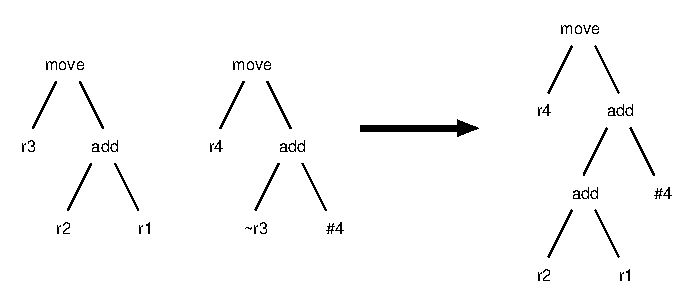
\includegraphics[height=3cm]{treegrow.eps}
\end{center}

\item Free {\tt r3} for duration, can be used for other purposes

\end{itemize}

\end{slide}


\begin{slide}

\heading{Concretisation}

\begin{itemize}
\item Join block body with head (control-flow instruction)
\item Perform instruction selection by dynamic programming
  \begin{itemize}
  \item Rule based; assigns cost for each rule
  \item Allows temporary creation when necessary
  \item Can cover any AST optimally
  \end{itemize}
\item Convert to binary code
\item Spit out of optimiser, replace original block(s)
\end{itemize}

\end{slide}


\begin{slide}

\heading{Register reallocation}

\begin{itemize}
\item Some transformations will generate new temporaries
\item Must assign to physical registers to make executable code
\item Allocate registers from pool:
  \begin{itemize}
  \item Registers freed by static analysis
  \item Registers freed by tree splicing
  \item `Stolen' registers
  \end{itemize}
\item Must avoid breaking global state
\end{itemize}

\end{slide}


\begin{slide}

\heading{Register stealing}

\begin{itemize}
\item Runtime system tracks live register set
\item Obtain registers for reallocation using heuristic:
  \begin{itemize}
  \item Live register set at start of a block is the same at optimisation time as it will be during future execution runs
  \end{itemize}
\item May prove to be untrue for different dynamic execution paths, so must be checked at runtime:
  \begin{itemize}
  \item (Live then AND NOT live now) != 0
  \end{itemize}
\item Fall back on old block if check fails
\end{itemize}

\end{slide}


\begin{slide}

\heading{Stack frame removal}

\begin{itemize}
\item May not be safe to remove register push \& pop from all dynamically-inlined functions
\item Easy for ``tail call'' type nested functions
\item Others by colouring stack code at compile time
\item Partly there already, can't prove it's safe though...
\end{itemize}

\end{slide}


\begin{slide}

\heading{Specialisation}

\begin{itemize}
\item Depends on heavyweight profiling
\item Can add a guard, rewrite a register at the start of a block with a constant value, then run optimisations
\item Constant propagation might cause beneficial cascading effects:
  \begin{itemize}
  \item Fixing loop iterations
  \item Deconditionalising branches
  \end{itemize}
\item Needs much more work...
\end{itemize}

\end{slide}

\end{document}
